\documentclass{beamer}

\usepackage[utf8]{inputenc}
\usepackage[spanish]{babel}
\usepackage{amsmath}
\usepackage[nosetup]{evan}
%\usetheme{Goddard}
\usetheme{Madrid}
\hypersetup{colorlinks,allcolors=.,urlcolor=magenta}
\usepackage[table]{xcolor} % Para definir colores en tablas
\usepackage{graphicx} % Para redimensionar la tabla
\usepackage{multicol}
\title[IO1]{Investigación de Operaciones I}
\subtitle{Método Simplex}
\author[Ricardo Largaespada]{Ricardo Jesús Largaespada Fernández}
\institute[UNI]{Ingeniería de Sistemas, DACTIC, UNI}
\date{06 de Septiembre, 2024}

\newenvironment<>{varblock}[2][.9\textwidth]{%
  \setlength{\textwidth}{#1}
  \begin{actionenv}#3%
    \def\insertblocktitle{#2}%
    \par%
    \usebeamertemplate{block begin}}
  {\par%
    \usebeamertemplate{block end}%
  \end{actionenv}}
  
\begin{document}

\frame{\titlepage}

\begin{frame}
\frametitle{Agenda}
\tableofcontents
\end{frame}

\begin{frame}
\frametitle{Introducción}
\begin{itemize}
    \item Vamos a estudiar cómo resolver un LP.
    \item El algoritmo que introduciremos es el método simplex.
    \begin{itemize}
        \item Desarrollado por \textbf{George Dantzig} en 1947.
        \item Abrió todo el campo de la Investigación de Operaciones.
        \item Implementado en la mayoría de los solucionadores comerciales de LP.
        \item Muy eficiente para casi todos los LP prácticos.
        \item Con ideas muy simples.
    \end{itemize}
    \item El método es general de manera indirecta.
    \begin{itemize}
        \item Hay muchas formas diferentes de LP.
        \item Primero mostraremos que cada LP es equivalente a un LP en \textbf{forma estándar}.
        \item Luego mostraremos cómo resolver LP en forma estándar.
    \end{itemize}
    \item ¡Esta clase estará llena de álgebra y teoremas. ¡Prepárate!
\end{itemize}
\end{frame}

\begin{frame}
\frametitle{Puntos extremos}
\begin{block}{Definición 1 (Puntos extremos)}
    Para un conjunto \(S \subseteq \mathbb{R}^n\), un punto \(x\) es un punto extremo si no existe un trío \((x^1, x^2, \lambda)\) tal que \(x^1 \in S \setminus \{x\}\), \(x^2 \in S \setminus \{x\}\), \(\lambda \in (0, 1)\), y 
    \[
    x = \lambda x^1 + (1- \lambda)x^2.
    \]
\end{block}
\begin{center}
    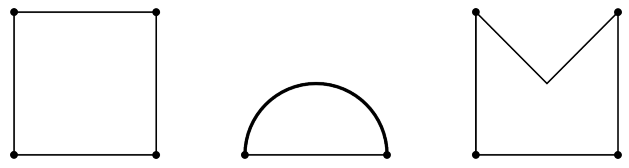
\includegraphics[width=6cm]{images/imagen_00.png}
\end{center}

\end{frame}

\begin{frame}
\frametitle{Optimalidad de los puntos extremos}

\begin{itemize}
    \item Para todos los LP, tenemos el siguiente hecho:
    \begin{block}{Proposición}
Para cualquier LP, si existe una solución óptima, existe una solución óptima en un punto extremo.
\end{block}
    \item No se está diciendo que ``si una solución es óptima, es un punto extremo''.
    \item Esta propiedad será muy útil cuando desarrollemos un método para resolver LPs generales.
\end{itemize}
\end{frame}

\section{Forma estándar de un LP}
\begin{frame}
\frametitle{Forma estándar de un LP}
\begin{block}{Definición 2 (LP en forma estándar)}
    Un LP está en forma estándar si:
    \begin{itemize}
        \item Todos los valores del lado derecho (RHS) son no negativos.
        \item Todas las variables son no negativas.
        \item Todas las restricciones son igualdades.
    \end{itemize}
\end{block}
\begin{itemize}
    \item RHS = right hand side. Para cualquier restricción
    \[g(x)\le b, g(x)\ge b, g(x)=b,\]
    \(b\) es el RHS.
    \item No hay restricción en la función objetivo.
\end{itemize}
\end{frame}

\subsection{Encontrando la forma estándar}
\begin{frame}
\frametitle{Encontrando la forma estándar}
\begin{itemize}
    \item ¿Cómo encontrar la forma estándar de un LP?
    \item Requisito 1: \textbf{RHS no negativo.}
    \begin{itemize}
        \item Si es negativo, \textbf{intercambie} el lado izquierdo (LHS) y el RHS.
        \item E.g. \[2x_1+3x_2\le -4\] es equivalente a \[-2x_1-3x_2\ge 4.\]
    \end{itemize}
\end{itemize}
\end{frame}

\begin{frame}
\frametitle{Encontrando la forma estándar}
\begin{itemize}
    \item Requisito 2: \textbf{Variables no negativas.}
    \begin{itemize}
        \item Si una variable es \textit{no positiva}, reemplácela por su negativo. E.g., \[2x_1+3x_2\le 4, x_1\le 0 \iff -2x_1+3x_2\le 4, x_1\ge 0.\]
        \item Si \(x_i\) es \textit{libre}, reemplácela por \(x_i'-x_i''\), donde \(x_i',x_i''\ge 0\). E.g.,
        \[2x_1+3x_2\le 4, x_1 \mbox{ sin rectricciones}\] \[\iff 2x_1'-2x_1''+3x_2\le 4, x_1',x_1'',x_2\ge 0.\]
        \[
\begin{array}{c|c|c}
x_i = x'_i - x''_i & x'_i \geq 0 & x''_i \geq 0 \\ \hline
5 & 5 & 0 \\
0 & 0 & 0 \\
-8 & 0 & 8 \\
\end{array}
\]
    \end{itemize}
\end{itemize}
\end{frame}

\begin{frame}
\frametitle{Encontrando la forma estándar}
\begin{itemize}
    \item Requisito 3: \textbf{Restricciones de igualdad.}
    \begin{itemize}
        \item Para una restricción ``\(\le\)'', agregue una \textit{variable de holgura}. E.g., \[2x_1+3x_2\le 4 \iff 2x_1+3x_2+x_3=4, x_3\ge 0.\]
        \item Para una restricción ``\(\ge\)'' resta una \textit{variable de exceso}. Por ejemplo:
\[
2x_1 + 3x_2 \geq 4 \quad \rightarrow \quad 2x_1 + 3x_2 - x_3 = 4; \quad x_3 \geq 0
\]
    \end{itemize}
    \item Para simplificar la exposición, ambos se llamarán variables de holgura.
    \item Una variable de holgura mide la diferencia entre el lado izquierdo (LHS) y el lado derecho (RHS) de la desigualdad.
\end{itemize}
\end{frame}

\begin{frame}{Un ejemplo}
\[
\begin{array}{cccccccc}
\text{min} & 3x_1& +& 2x_2& +& 4x_3& & \\
\text{s.a.} & x_1& +& 2x_2& -& x_3& \geq& 6 \\
 & -x_1& -& x_2& &&\geq& -8 \\
&2x_1& +& x_2& +& x_3& =& 9
\end{array}
\]
\[x_1 \geq 0, \, x_2 \leq 0, \, x_3 \text{ urs.}\]
\[
\Rightarrow
\begin{array}{cccccccccccccc}
\text{min} & 3x_1& -& 2x_2& +& 4x_3& -& 4x_4& &&&&&\\
\text{s.a.} & x_1& -& 2x_2& -& x_3& +& x_4& -& x_5& &&=& 6 \\
& x_1& -& x_2&&&&&&&+& x_6& =& 8 \\
& 2x_1& -& x_2& +& x_3& -& x_4&&&&&=& 9
\end{array}
\]
\[x_i \geq 0 \quad \forall i = 1, \ldots, 6.\]
\end{frame}

\subsection{LPs en forma estándar usando matrices}
\begin{frame}
\frametitle{LPs en forma estándar usando matrices}
\begin{itemize}
    \item Dado \textbf{cualquier} LP, podemos encontrar su forma estándar.
    \item Usando matrices, un LP en forma estándar se expresa como:
    \[
    \min \quad c^T x \quad \text{s.a.} \quad Ax = b, \quad x \geq 0.
    \]
    \item Por ejemplo, para
    \begin{multicols}{2}
    \[
    \min \quad 2x_1 - x_2
    \]
    \[
    \text{s.a.} \quad x_1 + 5x_2 + x_3 = 5
    \]
    \[
    3x_1 - 6x_2 + x_4 = 4
    \]
    \[
    x_i \geq 0 \quad \forall i = 1, \ldots, 4,
    \]
    \[
    c = \begin{bmatrix} 2 \\ -1 \\ 0 \\ 0 \end{bmatrix}, \quad b = \begin{bmatrix} 5 \\ 4 \end{bmatrix}, \quad \text{y}
    \]
    \[
    A = \begin{bmatrix} 1 & 5 & 1 & 0 \\ 3 & -6 & 0 & 1 \end{bmatrix}.
    \]
    \end{multicols}
    \item Denotaremos el número de restricciones y variables como \(m\) y \(n\).
    \begin{itemize}
        \item \(A \in \mathbb{R}^{m \times n}\) se llama \textbf{matriz de coeficientes}.
        \item \(b \in \mathbb{R}^m\) se llama \textbf{vector RHS (lado derecho)}.
        \item \(c \in \mathbb{R}^n\) se llama \textbf{vector objetivo}.
    \end{itemize}
    \item La función objetivo puede ser de maximización o minimización.
\end{itemize}
\end{frame}

\begin{frame}
\frametitle{Resolviendo LPs en forma estándar}
\begin{itemize}
    \item Entonces, ahora solo necesitamos encontrar una manera de resolver LPs en forma estándar.
    \item ¿Cómo?
    \item Un LP en forma estándar sigue siendo un LP.
    \item Si tiene una solución óptima, tiene una solución óptima en un \textbf{punto extremo}. ¡Por lo tanto, solo necesitamos buscar entre los puntos extremos!
\end{itemize}
\end{frame}

\section{Soluciones Básicas}
\begin{frame}
\frametitle{Soluciones básicas}
\begin{itemize}
    \item Consideremos un LP en forma estándar con \(m\) restricciones y \(n\) variables:
    \[
    \min \quad c^T x \quad \text{s.a.} \quad Ax = b, \quad x \geq 0.
    \]
    \item Podemos asumir que \(A\) tiene \(m\) pivotes, es decir, todas las filas de \(A\) son independientes.\footnote{Esta suposición se hace sin pérdida de generalidad. ¿Por qué?}
    \item Esto implica que \(m \leq n\). Dado que el problema con \(m = n\) es trivial, asumiremos que \(m < n\).
\end{itemize}
\end{frame}

\subsection{Definición}
\begin{frame}
\frametitle{Soluciones básicas}
\begin{itemize}
    \item Para el sistema \(Ax = b\), ahora hay más columnas que filas. Seleccionemos algunas columnas para formar una \textbf{solución básica}:

\begin{block}{Definición 3 (Solución básica)}
    Una solución básica para un LP en forma estándar es una solución que (1) tiene \(n - m\) variables iguales a 0 y (2) satisface \(Ax = b\).
\end{block}

\begin{itemize}
    \item Las \(n - m\) variables que se eligen para ser cero son \textbf{variables no básicas}.
    \item Las \(m\) variables restantes son \textbf{variables básicas}.
    \item El conjunto de variables básicas se llama una \textbf{base}.
    \item Estas \(m\) columnas forman una matriz \(m \times m\) no singular/invertible \(A_B\).
\end{itemize}
    
    \item Usamos \(x_B \in \mathbb{R}^m\) y \(x_N \in \mathbb{R}^{n-m}\) para denotar variables básicas y no básicas, respectivamente, con respecto a un conjunto dado de variables básicas \(B\).
    \begin{itemize}
        \item Tenemos \(x_N = 0\) y \(x_B = A_B^{-1}b\).
    \end{itemize}
\end{itemize}
\end{frame}

\subsection{Un ejemplo}
\begin{frame}
\frametitle{Soluciones básicas: un ejemplo}
\begin{multicols}{2}
\begin{itemize}
    \item Consideremos un LP original:
    \[
    \min \quad 6x_1 + 8x_2
    \]
    \[
    \text{s.a.} \quad x_1 + 2x_2 \leq 6
    \]
    \[
    2x_1 + x_2 \leq 6
    \]
    \[
    x_i \geq 0 \quad \forall i = 1, 2
    \]

    y su forma estándar:
    \[
    \min \quad 6x_1 + 8x_2
    \]
    \[
    \text{s.a.} \quad x_1 + 2x_2 + x_3 = 6
    \]
    \[
    2x_1 + x_2 + x_4 = 6
    \]
    \[
    x_i \geq 0 \quad \forall i = 1, \ldots, 4.
    \]
\end{itemize}
\end{multicols}
\begin{center}
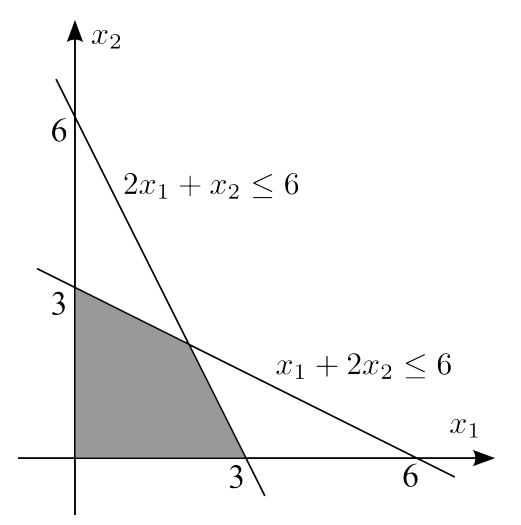
\includegraphics[width=4cm]{images/imagen_02.png}
\end{center}
\end{frame}

\begin{frame}
\frametitle{Soluciones básicas: un ejemplo}
\begin{itemize}
    \item En la forma estándar, \(m = 2\) y \(n = 4\).
    \begin{itemize}
        \item Hay \(n - m = 2\) variables no básicas.
        \item Hay \(m = 2\) variables básicas.
    \end{itemize}
    \item Pasos para obtener una solución básica:
    \begin{itemize}
        \item Determinar un conjunto de \(m\) variables básicas para formar una base \(B\).
        \item Las variables restantes forman el conjunto de variables no básicas \(N\).
        \item Establecer las variables no básicas en cero: \(x_N = 0\).
        \item Resolver el sistema \(m \times m\) \(A_B x_B = b\) para obtener los valores de las variables básicas.
    \end{itemize}
    \item Para este ejemplo, resolveremos un sistema de dos por dos para cada base.
\end{itemize}
\end{frame}

\begin{frame}
\frametitle{Soluciones básicas: un ejemplo}
\begin{itemize}
    \item Las dos igualdades son:
    \[
    \begin{array}{rcl}
    x_1 + 2x_2 + x_3 & = & 6 \\
    2x_1 + x_2 + x_4 & = & 6.
    \end{array}
    \]
    \item Intentemos con \(B = (x_1, x_2)\) y \(N = (x_3, x_4)\):
    \[
    \begin{array}{rcl}
    x_1 + 2x_2 & = & 6 \\
    2x_1 + x_2 & = & 6.
    \end{array}
    \]
    La solución es \((x_1, x_2) = (2, 2)\). Por lo tanto, la solución básica asociada con esta base \(B\) es \((x_1, x_2, x_3, x_4) = (2, 2, 0, 0)\).
    \item Intentemos con \(B = (x_2, x_3)\) y \(N = (x_1, x_4)\):
    \[
    \begin{array}{rcl}
    2x_2 + x_3 & = & 6 \\
    x_2 & = & 6.
    \end{array}
    \]
    Como \((x_2, x_3) = (6, -6)\), la solución básica es \((x_1, x_2, x_3, x_4) = (0, 6, -6, 0)\).
\end{itemize}
\end{frame}

\begin{frame}
\frametitle{Soluciones básicas: un ejemplo}
\begin{itemize}
    \item En general, dado que necesitamos elegir \(m\) de entre \(n\) variables para que sean básicas, tenemos como máximo \(\binom{n}{m}\) bases diferentes.\footnote{¿Por qué ``como máximo''? ¿Por qué no ``exactamente''?}
    \item En este ejemplo, tenemos exactamente \(\binom{4}{2} = 6\) bases.
    \item Examinando las seis bases una por una, podemos encontrar todas las variables básicas asociadas:
\end{itemize}

\begin{center}
\begin{tabular}{c|cccc}
    \(B\) & \multicolumn{4}{c}{Solución básica} \\
    & \(x_1\) & \(x_2\) & \(x_3\) & \(x_4\) \\ \hline
    \((x_1, x_2)\) & 2 & 2 & 0 & 0 \\
    \((x_1, x_3)\) & 3 & 0 & 3 & 0 \\
    \((x_1, x_4)\) & 6 & 0 & 0 & -6 \\
    \((x_2, x_3)\) & 0 & 6 & -6 & 0 \\
    \((x_2, x_4)\) & 0 & 3 & 0 & 3 \\
    \((x_3, x_4)\) & 0 & 0 & 6 & 6 \\
\end{tabular}
\end{center}

\end{frame}

\subsection{Solución Básica Factible}

\begin{frame}
\frametitle{Soluciones básicas factibles}
\begin{itemize}
    \item Entre todas las soluciones básicas, algunas son factibles.
    \begin{itemize}
        \item Según la definición de soluciones básicas, estas satisfacen \(Ax = b\).
        \item Si además satisfacen \(x \geq 0\), satisfacen todas las restricciones.
    \end{itemize}
    \item En este caso, se llaman \textbf{soluciones básicas factibles} (bfs).
\end{itemize}
\begin{multicols}{2}
    \begin{varblock}[6cm]{Definición 4 (Solución básica factible)}
    Una solución básica factible para un LP en forma estándar es una solución básica cuyas variables básicas son todas no negativas.
\end{block}

\begin{itemize}
    \item ¿Cuáles son bfs?
\end{itemize}

\begin{center}
\begin{tabular}{c|cccc}
    Base & \multicolumn{4}{c}{Solución básica} \\
    & \(x_1\) & \(x_2\) & \(x_3\) & \(x_4\) \\ \hline
    \((x_1, x_2)\) & 2 & 2 & 0 & 0 \\
    \((x_1, x_3)\) & 3 & 0 & 3 & 0 \\
    \((x_1, x_4)\) & 6 & 0 & 0 & -6 \\
    \((x_2, x_3)\) & 0 & 6 & -6 & 0 \\
    \((x_2, x_4)\) & 0 & 3 & 0 & 3 \\
    \((x_3, x_4)\) & 0 & 0 & 6 & 6 \\
\end{tabular}
\end{center}
\end{multicols}

\end{frame}

\subsection{bfs y puntos extremos}
\begin{frame}
\frametitle{Soluciones básicas factibles y puntos extremos}
\begin{itemize}
    \item ¿Por qué son importantes las bfs? ¡Simplemente son puntos extremos!
\end{itemize}

\begin{block}{Teorema 1 (Puntos extremos y soluciones básicas factibles)}
    Para un LP en forma estándar, una solución es un punto extremo de la región factible si y solo si es una solución básica factible del LP.
\end{block}

\begin{itemize}
    \item La implicación es directa:
\end{itemize}

\begin{block}{Teorema 2 (Optimalidad de las soluciones básicas factibles)}
    Para un LP en forma estándar, si existe una solución óptima, existe una solución básica factible óptima.
\end{block}

\begin{itemize}
    \item Aunque no podemos demostrar el Teorema 1 aquí, obtengamos algunas intuiciones.\footnote{Tenga en cuenta que estas ``intuiciones'' nunca son rigurosas.}
\end{itemize}

\end{frame}

\begin{frame}
\frametitle{Un ejemplo}
\begin{itemize}
    \item Hay una correspondencia uno a uno entre las bfs y los puntos extremos.
\end{itemize}
\begin{multicols}{2}
\begin{center}
\begin{tabular}{c|c|c|cccc}
    Base & ¿Bfs? & Punto & \multicolumn{4}{c}{Solución básica} \\
    & & & \(x_1\) & \(x_2\) & \(x_3\) & \(x_4\) \\ \hline
    \((x_1, x_2)\) & Sí & \textcolor{blue}{A} & 2 & 2 & 0 & 0 \\
    \((x_1, x_3)\) & Sí & \textcolor{blue}{B} & 3 & 0 & 3 & 0 \\
    \((x_1, x_4)\) & No & C & 6 & 0 & 0 & -6 \\
    \((x_2, x_3)\) & No & D & 0 & 6 & -6 & 0 \\
    \((x_2, x_4)\) & Sí & \textcolor{blue}{E} & 0 & 3 & 0 & 3 \\
    \((x_3, x_4)\) & Sí & \textcolor{blue}{F} & 0 & 0 & 6 & 6 \\
\end{tabular}
\end{center}

\begin{center}
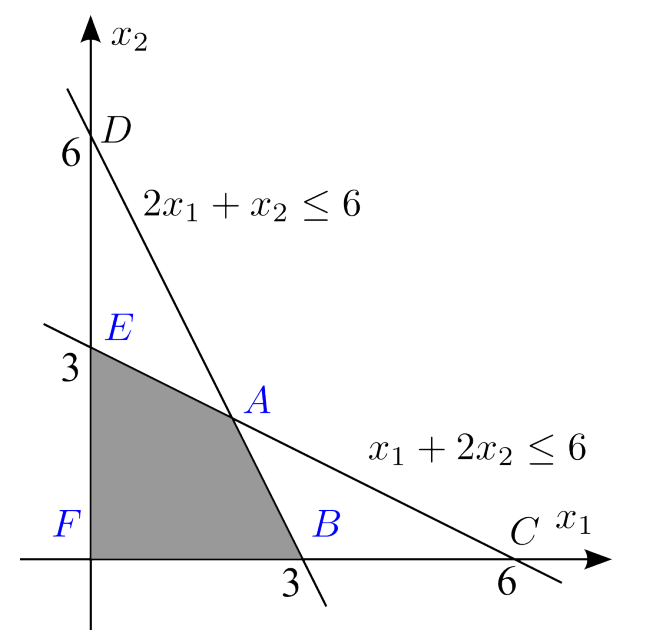
\includegraphics[width=3.5cm]{images/imagen_03.png}
\end{center}
\end{multicols}
\end{frame}

\begin{frame}
\frametitle{Resolviendo LPs en forma estándar}
\begin{itemize}
    \item Para encontrar una solución óptima:
    \begin{itemize}
        \item En lugar de buscar entre todos los puntos extremos, buscamos entre todas las bfs.
        \item Los puntos extremos se definen geométricamente; las bfs son algebraicas.
        \item Verificar si una solución es básica factible es fácil (para una computadora).
    \end{itemize}
    \item Para buscar entre las bfs, seguimos moviéndonos a una bfs adyacente mejor desde la actual:
\end{itemize}

\begin{block}{Definición 5 (Bases adyacentes y bfs)}
    Dos bases son adyacentes si exactamente una de sus variables es diferente. Dos bfs son adyacentes si sus bases asociadas son adyacentes.
\end{block}

\begin{itemize}
    \item Nuevamente, usemos un gráfico para entender la idea.
\end{itemize}

\end{frame}

\begin{frame}
\frametitle{Soluciones básicas factibles adyacentes}
\begin{itemize}
    \item Un par de bfs adyacentes corresponde a un par de puntos extremos ``adyacentes'', es decir, puntos extremos que están en la misma arista.
    \item Cambiar de una bfs a su bfs adyacente es moverse a lo largo de una arista.
\end{itemize}
\begin{multicols}{2}
\begin{center}
\begin{tabular}{c|c|c|cccc}
    Base & Punto & \multicolumn{4}{c}{Solución básica} \\
    & & \(x_1\) & \(x_2\) & \(x_3\) & \(x_4\) \\ \hline
    \((x_1, x_2)\) & A & 2 & 2 & 0 & 0 \\
    \((x_1, x_3)\) & \textcolor{blue}{B} & 3 & 0 & 3 & 0 \\
    \((x_2, x_4)\) & E & 0 & 3 & 0 & 3 \\
    \((x_3, x_4)\) & \textcolor{blue}{F} & 0 & 0 & 6 & 6 \\
\end{tabular}
\end{center}

\begin{center}
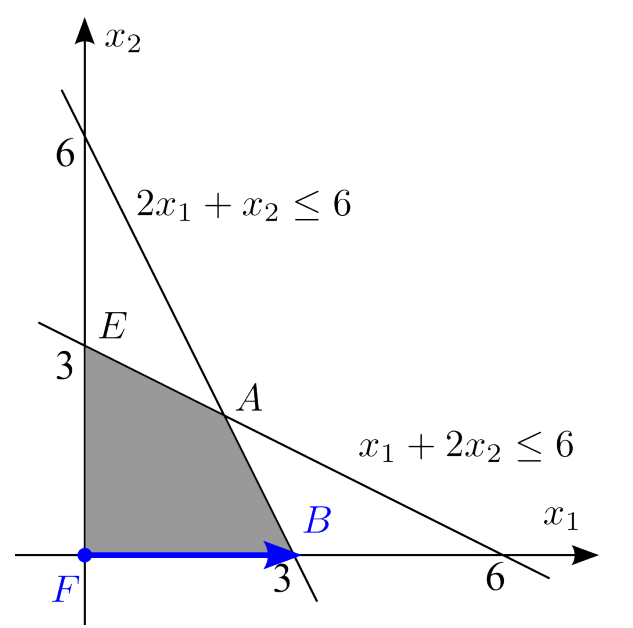
\includegraphics[width=0.45\textwidth]{images/imagen_04.png}
\end{center}
\end{multicols}
\end{frame}

\begin{frame}
\frametitle{Una mejor manera de buscar}
\begin{itemize}
    \item Dados todos estos conceptos, ¿cómo buscarías entre las bfs?
    \item En cada bfs, muévete a una bfs adyacente que sea mejor.
    \begin{itemize}
        \item Alrededor de la bfs actual, debería haber algunas direcciones de mejora.
        \item De lo contrario, la bfs es óptima.
    \end{itemize}
    \item A continuación, introduciremos el método simplex, que utiliza esta idea de una manera elegante.
\end{itemize}
\end{frame}

\section{El Método Simplex}
\subsection{La idea}
\begin{frame}
\frametitle{La idea}
\begin{itemize}
    \item Todo lo que necesitamos es buscar entre las bfs.
    \begin{itemize}
        \item Geométricamente, buscamos entre los puntos extremos.
        \item Moverse a una bfs adyacente es moverse a lo largo de una arista.
    \end{itemize}
    \item Preguntas:
    \begin{itemize}
        \item ¿Por qué arista moverse?
        \item ¿Cuándo dejar de moverse?
    \end{itemize}
    \item Todo esto debe hacerse con álgebra en lugar de geometría.
    \item Algebraicamente, para moverse a una bfs adyacente, necesitamos reemplazar una variable básica por una variable no básica.
    \begin{itemize}
        \item Por ejemplo, moverse de \(B_1 = (x_1, x_2, x_3)\) a \(B_2 = (x_2, x_3, x_5)\).
    \end{itemize}
    \item Hay dos cosas que hacer:
    \begin{itemize}
        \item Seleccionar una variable no básica para entrar en la base, y
        \item Seleccionar una variable básica para salir de la base.
    \end{itemize}
\end{itemize}
\end{frame}

\begin{frame}
\frametitle{La idea}
\begin{itemize}
    \item Entrar y salir:
    \begin{itemize}
        \item Seleccionar una variable no básica para entrar significa hacerla diferente de cero: aumentar su valor de 0 a un valor positivo y convertirla en básica.
        \item Mientras esta variable aumenta, identificamos las variables básicas que disminuyen y nos detenemos cuando una de ellas llega a 0. Esa variable sale de la base y se convierte en no básica.
    \end{itemize}
    \item Seguimos cambiando la base hasta encontrar una base óptima.
    \item A continuación, aprendamos exactamente cómo ejecutar el método simplex en álgebra.
\end{itemize}
\end{frame}

\subsection{El primer movimiento}
\begin{frame}
\frametitle{El método simplex}
\begin{itemize}
    \item Para introducir el álgebra del método simplex, consideremos el siguiente LP:
    \[
    \begin{array}{ll}
    \text{max} & 2x_1 + 3x_2 \\
    \text{s.a.} & x_1 + 2x_2 \leq 6 \\
    & 2x_1 + x_2 \leq 8 \\
    & x_i \geq 0 \quad \forall i = 1, 2
    \end{array}
    \]
    \item y su forma estándar:
    \[
    \begin{array}{ll}
    \text{max} & 2x_1 + 3x_2 \\
    \text{s.a.} & x_1 + 2x_2 + x_3 = 6 \\
    & 2x_1 + x_2 + x_4 = 8 \\
    & x_i \geq 0 \quad \forall i = 1, \ldots, 4.
    \end{array}
    \]
\end{itemize}
\end{frame}

\begin{frame}
\frametitle{Sistema de igualdades}
\begin{itemize}
    \item Necesitamos llevar un seguimiento del valor objetivo.
    \begin{itemize}
        \item Queremos seguir mejorando nuestra solución.
        \item Usaremos \(z = 2x_1 + 3x_2\) para denotar el valor objetivo.
        \item El valor objetivo a veces se llamará el valor \(z\).
    \end{itemize}
    \item Una vez que recordamos que (1) estamos maximizando \(z\) y (2) todas las variables (excepto \(z\)) deben ser no negativas, la forma estándar no es más que un sistema de tres igualdades:
    \[
    \begin{array}{rcl}
    z - 2x_1 - 3x_2 & = & 0 \\
    x_1 + 2x_2 + x_3 & = & 6 \\
    2x_1 + x_2 + x_4 & = & 8.
    \end{array}
    \]
    \item Nota que \(z = 2x_1 + 3x_2\) se expresa como \(z - 2x_1 - 3x_2 = 0\).
    \item Esta ``restricción'' (que en realidad representa la función objetivo) se llamará la restricción 0.
    \item Repetidamente resolveremos el sistema.
\end{itemize}
\end{frame}

\begin{frame}
\frametitle{Una bfs inicial}
\begin{itemize}
    \item Para comenzar, primero necesitamos tener una bfs inicial.
    \item Investigamos el sistema en detalle:
    \[
    \begin{array}{rcl}
    z - 2x_1 - 3x_2 & = & 0 \\
    x_1 + 2x_2 + x_3 & = & 6 \\
    2x_1 + x_2 + x_4 & = & 8.
    \end{array}
    \]
    \begin{itemize}
        \item ¡Seleccionar \(x_3\) y \(x_4\) definitivamente funciona!
        \item En el sistema, estas dos columnas forman una matriz identidad: \(A_B = I\).\footnote{Para la mayoría de los LPs, tal matriz identidad no existe. Veremos cómo lidiar con esta situación.}
        \item Además, en un LP en forma estándar, los términos del lado derecho (RHS) \(b\) son no negativos.
        \item Por lo tanto, \(x_B = A_B^{-1}b = Ib = b \geq 0\).
    \end{itemize}
\end{itemize}
\end{frame}

\begin{frame}
\frametitle{Mejorando la bfs actual}
\[
\begin{array}{rcl}
z - 2x_1 - 3x_2 & = & 0 \\
x_1 + 2x_2 + x_3 & = & 6 \\
2x_1 + x_2 + x_4 & = & 8.
\end{array}
\]
\begin{itemize}
    \item Comencemos desde \(x^1 = (0, 0, 6, 8)\) y \(z_1 = 0\).
    \item Para movernos, elijamos una variable no básica para entrar. ¿\(x_1\) o \(x_2\)?
    \begin{itemize}
        \item La restricción 0 nos dice que entrar cualquier variable hace que \(z\) aumente: cuando una sube, \(z\) sube para mantener la igualdad.
        \item Sin razón en particular, elijamos que \(x_1\) entre.
    \end{itemize}
    \item ¿Cuándo detenernos?
    \begin{itemize}
        \item Ahora \(x_1\) sube desde 0.
        \item \( (0, 0, 6, 8) \rightarrow (1, 0, 5, 6) \rightarrow (2, 0, 4, 4) \rightarrow \cdots \). Nota que \(x_2\) permanece en 0.
        \item Nos detendremos en \( (4, 0, 2, 0) \), es decir, cuando \(x_4\) se vuelve 0.
        \item Esto está indicado por la razón del RHS y la columna que entra: \( \frac{8}{2} < \frac{6}{1} \); \(x_4\) se vuelve 0 antes que \(x_3\).
    \end{itemize}
    \item Nos movemos a \(x^2 = (4, 0, 2, 0)\) con \(z_2 = 8\).
\end{itemize}
\end{frame}

\subsection{El segundo movimiento}
\begin{frame}
\frametitle{Seguir mejorando la bfs actual}
\begin{itemize}
    \item Mejoremos \(x^2 = (4, 0, 2, 0)\) moviéndonos a la siguiente bfs.
    \begin{itemize}
        \item Uno de \(x_2\) y \(x_4\) puede entrar. Intentemos con \(x_2\).
    \end{itemize}
    \item Cuando \(x_2\) sube y \(x_4\) permanece en 0:
    \begin{itemize}
        \item La segunda fila dice que \(x_2\) puede llegar a ser como máximo 8 (y entonces \(x_1\) se vuelve 0).
        \item En la primera fila... ¿cómo cambiarán \(x_1\) y \(x_3\)?
    \end{itemize}
    \item De acuerdo con la restricción 2, cuando \(x_2\) sube 1 y \(x_4\) permanece en 0, \(x_1\) debe disminuir en \(\frac{1}{2}\).
    \begin{itemize}
        \item Por lo tanto, según la restricción 1, cuando \(x_2\) sube 1 ``y'' \(x_1\) baja en \(\frac{1}{2}\), \(x_3\) debería bajar en \(\frac{3}{2}\).
        \item Por lo tanto, \(x_2\) puede ser como máximo \(\frac{4}{3}\). Alcanzamos \( \left(\frac{10}{3}, \frac{4}{3}, 0, 0\right)\).
    \end{itemize}
    \item Colectivamente, deberíamos aumentar \(x_2\) por \(\min\left\{8, \frac{4}{3}\right\}\).
    \begin{itemize}
        \item El valor de \(z\) se convierte en \(z_3 = \frac{10}{3} \times 2 + \frac{4}{3} \times 3 = \frac{32}{3}\).
        \item No se convierte en \(z_2 + \frac{4}{3} \times 3\) ya que la variable básica \(x_1\) también cambia.
    \end{itemize}
\end{itemize}
\end{frame}

\begin{frame}
\frametitle{Seguir mejorando la bfs actual}
\begin{itemize}
    \item Nota que lo que hicimos tiene dos defectos.
    \item Con respecto a las restricciones:
    \begin{itemize}
        \item Cuando aumentamos la variable no básica \(x_2\), puede afectar a las variables básicas \(x_1\) y \(x_3\).
        \item Debido a que \(x_3\) no aparece en la restricción 2, sabemos cómo responde \(x_1\) al cambio de \(x_2\).
        \item Necesitamos considerar eso para ver cómo \(x_3\) responde al cambio de \(x_2\).
    \end{itemize}
    \item Con respecto a la función objetivo:
    \begin{itemize}
        \item Cuando aumentamos la variable no básica \(x_2\), afecta a las variables básicas \(x_1\) y \(x_3\).
        \item Debido a que \(x_1\) está en la restricción 0, \(z\) se ve afectado tanto por \(x_1\) como por \(x_2\).
    \end{itemize}
    \item ¿Cómo hacer estos cálculos con miles de variables y restricciones?
\end{itemize}
\end{frame}

\subsection{Actualización del sistema mediante operaciones elementales de fila.}
\begin{frame}
\frametitle{Seguir mejorando la bfs actual}
\[
\begin{array}{rcl}
z - 2x_1 - 3x_2 & = & 0 \\
x_1 + 2x_2 + x_3 & = & 6 \\
2x_1 + x_2 + x_4 & = & 8.
\end{array}
\]
\begin{itemize}
    \item Una manera más fácil es actualizar el sistema antes del segundo movimiento.
    \begin{itemize}
        \item Hacer que cada una de las filas 1 a \(n\) contenga exactamente una variable básica.
        \item Hacer que la fila 0 no contenga ninguna variable básica.
    \end{itemize}
    \item En otras palabras, para las columnas básicas:
    \begin{itemize}
        \item Queremos una matriz identidad en las filas 1 a \(m\).
        \item Queremos un vector cero en la fila 0.
    \end{itemize}
\end{itemize}
\end{frame}

\begin{frame}
\frametitle{Mejorando la bfs actual (segundo intento)}
\begin{itemize}
    \item Recordemos que para el sistema
    \[
    \begin{array}{rcl}
    z - 2x_1 - 3x_2 & = & 0 \\
    x_1 + 2x_2 + x_3 & = & 6 \\
    2x_1 + x_2 + x_4 & = & 8,
    \end{array}
    \]
    comenzamos con \(x^1 = (0, 0, 6, 8)\) con \(z_1 = 0\).
    \begin{itemize}
        \item Para las columnas básicas (las 3ra y 4ta), de hecho tenemos la matriz identidad y ceros.
    \end{itemize}
    \item Entonces sabemos que \(x_1\) entra y \(x_4\) sale.
    \begin{itemize}
        \item La base se convierte en \((x_1, x_3)\).
        \item Necesitamos actualizar el sistema a
    \end{itemize}
\begin{center}
    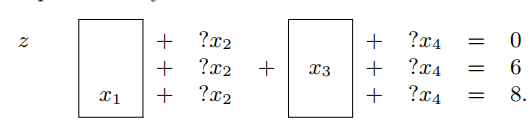
\includegraphics[width=6cm]{images/imagen_05.png}
\end{center}
    \item ¿Cómo? ¡Operaciones elementales de fila!
\end{itemize}
\end{frame}

\begin{frame}
\frametitle{Actualizando el sistema}
\begin{itemize}
    \item Partiendo de:
    \[
    \begin{array}{rcl}
    z - 2x_1 - 3x_2 & = & 0 \quad \text{(0)} \\
    x_1 + 2x_2 + x_3 & = & 6 \quad \text{(1)} \\
    2x_1 + x_2 + x_4 & = & 8 \quad \text{(2)}
    \end{array}
    \]
    \begin{itemize}
        \item Multiplica (2) por \(\frac{1}{2}\): \(x_1 - \frac{1}{2}x_2 + \frac{1}{2}x_4 = 4\).
        \item Multiplica (2) por \(-\frac{1}{2}\) y luego súmalo a (1): \(\frac{3}{2}x_2 + x_3 - \frac{1}{2}x_4 = 2\).
        \item Multiplica (2) por 1 y luego súmalo a (0): \(z - 2x_2 + x_4 = 8\).
    \end{itemize}
    \item Colectivamente, el sistema se convierte en:
    \[
    \begin{array}{ccccccccccc}
    z&&&-&2x_2&&&+&x_4&=&8\\
    &&&&\frac{3}{2}x_2&+&x_3&-&\frac{1}{2}x_4&=&2\\
    &&x_1&+&\frac{1}{2}x_2&&&+&\frac{1}{2}x_4&=&4.\\
    \end{array}
    \]
    \item Actualizar el sistema también nos da el valor objetivo \(z_2 = 8\) y la bfs actual \(x^2 = (4, 0, 2, 0)\).
\end{itemize}
\end{frame}

\begin{frame}
\frametitle{Mejorando la bfs actual (¡finalmente!)}
\begin{itemize}
    \item Dado el sistema actualizado:
    \[
    \begin{array}{rcl}
    z - 2x_2 + x_4 & = & 8 \quad \text{(0)} \\
    \frac{3}{2}x_2 + x_3 - \frac{1}{2}x_4 & = & 2 \quad \text{(1)} \\
    x_1 + \frac{1}{2}x_2 + \frac{1}{2}x_4 & = & 4, \quad \text{(2)}
    \end{array}
    \]
    ahora sabemos cómo hacer la siguiente iteración.
    \begin{itemize}
        \item Estamos en \(x^2 = (4, 0, 2, 0)\) con \(z_2 = 8\).
        \item Uno de \(x_2\) y \(x_4\) puede entrar.
        \item Si entra \(x_2\), \(z\) subirá. ¡Bien!
        \item Si entra \(x_4\), \(z\) bajará. Malo.
    \end{itemize}
    \item Dejemos que \(x_2\) entre:
    \begin{itemize}
        \item Fila 1: Cuando \(x_2\) sube, \(x_3\) baja. \(x_2\) puede ser tan grande como \(\frac{2}{\frac{3}{2}} = \frac{4}{3}\).
        \item Fila 2: Cuando \(x_2\) sube, \(x_1\) baja. \(x_2\) puede ser tan grande como \(\frac{4}{\frac{1}{2}} = 8\).
        \item Entonces, \(x_3\) se convierte en 0 antes que \(x_1\). \(x_3\) sale de la base.
    \end{itemize}
    \item Las variables básicas se convierten en \(x_1\) y \(x_2\). Actualicemos de nuevo.
\end{itemize}
\end{frame}

\subsection{El último intento sin más mejora.}
\begin{frame}
\frametitle{Mejorando una vez más}
\begin{itemize}
    \item Dado el sistema:
    \[
    \begin{array}{rcl}
    z - 2x_2 + x_4 & = & 8 \quad \text{(0)} \\
    \frac{3}{2}x_2 + x_3 - \frac{1}{2}x_4 & = & 2 \quad \text{(1)} \\
    x_1 + \frac{1}{2}x_2 + \frac{1}{2}x_4 & = & 4, \quad \text{(2)}
    \end{array}
    \]
    ahora necesitamos actualizarlo para ajustarlo a la nueva base \((x_1, x_2)\).
    \begin{itemize}
        \item Multiplica (1) por \(\frac{2}{3}\): \(x_2 + \frac{2}{3}x_3 - \frac{1}{3}x_4 = \frac{4}{3}\).
        \item Multiplica (la actualizada) (1) por \(-\frac{1}{2}\) y súmala a (2).
        \item Multiplica (la actualizada) (1) por 2 y súmala a (0).
    \end{itemize}
    \item Obtenemos:
    \[
    \begin{array}{rcl}
    z + \frac{4}{3}x_3 + \frac{1}{3}x_4 & = & \frac{32}{3} \quad \text{(0)} \\
    x_2 + \frac{2}{3}x_3 - \frac{1}{3}x_4 & = & \frac{4}{3} \quad \text{(1)} \\
    x_1 - \frac{1}{3}x_3 + \frac{2}{3}x_4 & = & \frac{10}{3}. \quad \text{(2)}
    \end{array}
    \]
\end{itemize}
\end{frame}

\begin{frame}
\frametitle{¡No más mejoras!}
\begin{itemize}
    \item El sistema
    \[
    \begin{array}{rcl}
    z + \frac{4}{3}x_3 + \frac{1}{3}x_4 & = & \frac{32}{3} \quad \text{(0)} \\
    x_2 + \frac{2}{3}x_3 - \frac{1}{3}x_4 & = & \frac{4}{3} \quad \text{(1)} \\
    x_1 - \frac{1}{3}x_3 + \frac{2}{3}x_4 & = & \frac{10}{3} \quad \text{(2)}
    \end{array}
    \]
    nos dice que la nueva bfs es \(x^3 = \left(\frac{10}{3}, \frac{4}{3}, 0, 0\right)\) con \(z_3 = \frac{32}{3}\).
    \begin{itemize}
        \item Actualizar el sistema también nos da la nueva bfs y su valor objetivo.
    \end{itemize}
    \item Ahora... ¡no se necesita más mejora!
    \begin{itemize}
        \item Si entra \(x_3\), las cosas empeoran (z debe bajar).
        \item Si entra \(x_4\), también las cosas empeoran.
    \end{itemize}
    \item \(x^3\) es una solución óptima.\footnote{Esto es realmente cierto, aunque se omite una demostración rigurosa.} ¡Hemos terminado!
\end{itemize}
\end{frame}

\subsection{Visualización y resumen del método simplex.}
\begin{frame}
\frametitle{Visualizando las iteraciones}
\begin{itemize}
    \item Visualicemos este ejemplo y relacionemos las bfs con los puntos extremos.
    \begin{itemize}
        \item La bfs inicial corresponde a \((0, 0)\).
        \item Después de una iteración, nos movemos a \((4, 0)\).
        \item Después de dos iteraciones, nos movemos a \(\left(\frac{10}{3}, \frac{4}{3}\right)\), que es óptima.
    \end{itemize}
    \item ¡Por favor, note que nos movemos a lo largo de aristas para buscar entre los puntos extremos!
\end{itemize}

\begin{center}
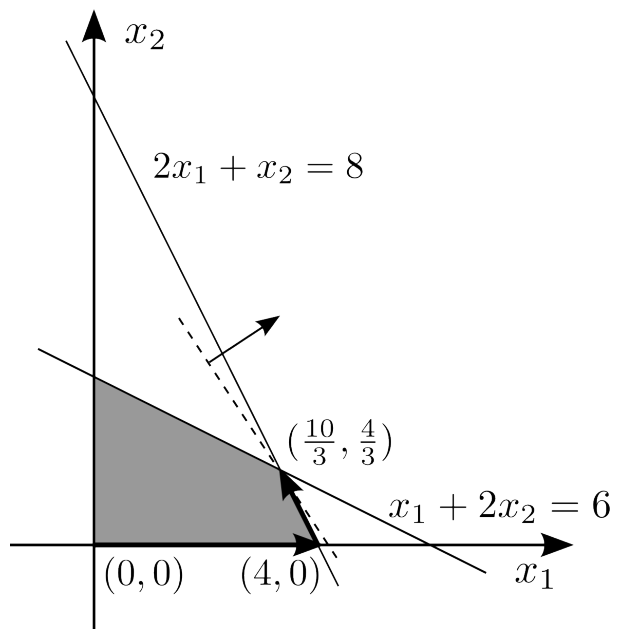
\includegraphics[width=5cm]{images/imagen_06.png}
\end{center}

\end{frame}

\begin{frame}
\frametitle{Resumen}
\begin{itemize}
    \item Para ejecutar el método simplex:
    \begin{itemize}
        \item Encuentra una bfs inicial con su base.\footnote{¿Cómo encontrar una?}
        \item Entre aquellas variables no básicas con coeficientes positivos en la fila 0,\footnote{Coeficientes positivos para un problema de minimización; negativos para maximización.} elige una para entrar.\footnote{¿Qué pasa si hay múltiples?}
        \begin{itemize}
            \item Si no hay ninguna, termina e informa la bfs actual como óptima.
        \end{itemize}
        \item De acuerdo con las razones entre las columnas de entrada y el lado derecho, decide qué variable básica debe salir.\footnote{¿Qué pasa si hay un empate? ¿Qué pasa si el denominador es 0 o negativo?}
        \item Encuentra una nueva base.
        \item Ajusta el sistema para cumplir con los requisitos de las columnas básicas:
        \begin{itemize}
            \item Matriz identidad en las restricciones (de la fila 1 a la \(m\)).
            \item Ceros en la función objetivo (fila 0).
        \end{itemize}
        \item Repite.
    \end{itemize}
\end{itemize}
\end{frame}

\end{document}